\newpage
\section{Iteración 1: Prototipo del robot}

\subsection{Introducción}
En la iteración anterior obtuvimos como resultado los principios y bases fundamentales sobre las que desarrollaremos esta iteración para lograr un prototipo funcional.

\subsection{Requerimientos}
En esta iteración abordaremos los siguientes requerimientos funcionales:

\begin{center} \begin{tabular}{|c|c|}
\hline
    ID & Descripción \\
\hline
    RF1 & El robot debe contar con un sistema de control para las 4 ruedas. \\ 
\hline
    RF2 & El robot debe tener un sistema de locomoción omnidireccional. \\ 
\hline
    RF3 & El robot debe poder medir la distancia recorrida. \\ 
\hline
    RF4 & El robot debe poder realizar trayectorias en línea recta y curvas. \\ 
\hline
    RF5 & El robot debe poder corregir su trayectoria mediante el uso de sensores. \\  
\hline
    RF6 & El robot debe recibir y enviar información mediante comunicaciones inalámbricas. \\ 
\hline
\end{tabular} \end{center}

Por otra parte, los requerimientos no funcionales que trataremos son:

\begin{center} \begin{tabular}{|p{0.10\linewidth}|p{0.65\linewidth}|}
\hline
    ID & Descripción \\
\hline
    RNF1 & Debería tener tiempos de respuesta aceptables para el buen funcionamiento del sistema de control. \\
\hline
    RNF2 & El software debería contar con pruebas unitarias y de integración. \\
\hline
    RNF4 & El código debería contar con documentación.\\
\hline
\end{tabular} \end{center}

\subsection{Desarrollo}

\subsubsection{Sistema de control PID}
Un controlador PID (Proporcional-Integral-Derivativo) es un tipo de controlador utilizado en sistemas de control automático para mantener una variable de algún proceso lo más cercana posible a un valor deseado, conocido como "setpoint", a pesar de las perturbaciones encontradas. La acción proporcional responde al error actual, que es la diferencia entre el valor deseado y el valor medido, ajustando la salida del controlador proporcionalmente a este error. Por otro lado, la acción integral se enfoca en la acumulación de errores pasados para eliminar cualquier error que sea persistente, asegurando que con el tiempo la variable de proceso converja al setpoint establecido. Finalmente, la acción derivativa considera la tasa de cambio del error, anticipando y corrigiendo cualquier futura tendencia del error, sumando a la estabilidad del sistema.

El objetivo principal de un controlador PID es proporcionar una respuesta rápida y estable en diferentes aplicaciones. Además de ser utilizado en procesos industriales como plantas químicas y refinerías, también se lo utiliza en el control de velocidad de motores eléctricos, asegurando que el motor funcione a la velocidad deseada sin fluctuaciones por mas que se perciban alteraciones, por lo que en robótica resultan útiles para el control de posición y movimiento, permitiendo acciones precisas y controladas.

\paragraph{Función de transferencia del motor} \mbox{} \vspace{8pt}

La función de transferencia en un sistema de control se representa como $G(s)$ y modela matemáticamente el comportamiento de un actuador, al cual se le aplica un estimulo o señal $R(s)$ y se obtiene una respuesta $C(s)$ por parte de él.

Para controlar la variable en cuestión debemos tener una noción sobre la salida producida. Por un lado tenemos la función $H(s)$, que es una función que toma como entrada una medición sobre la salida del actuador o sistema para producir un valor $B(s)$. Éste se suma negativamente al setpoint $R(s)$ para obtener el error entre ellas $E(s)$, que es la señal efectivamente que se introduce a $G(s)$ para logar aproximarse al setpoint y compensar el sistema.

\begin{figure}[H]
    \centering
    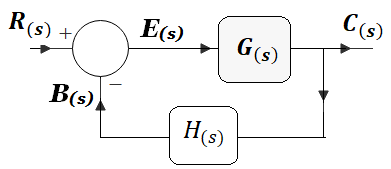
\includegraphics[width=0.4\linewidth]{sistema_de_control}
    \caption{Sistema de control realimentado}
    \label{fig:sistcontrolrealim}
\end{figure}

Para lograr controlar cada motor de cada rueda es necesario conocer la función de transferencia del mismo para lograr modelarlo. Al no contar con la hoja de datos del fabricante por ser un motor genérico, se realizaron una serie de experimentos para aproximar la función $G(s)$. En nuestro caso debemos obtener una función de transferencia que tenga como entrada $[Volts]$ y su salida sea $[RPM]$.

Para hacer esto se propone hacer uso del método de la constante de tiempo $\tau$. En primer lugar, consideraremos que la curva alcanza el $63.2\%$  del valor final cuando ha transcurrido un tiempo $t=\tau$. En la gráfica el valor final de la curva es 1, es decir, $y(\infty)=1$. Por lo que debemos identificar el instante $t$ para el cual se cumple que $y(t)=0.632$.

El paso siguiente es trazar una recta paralela al eje de las abscisas (eje $t$) que corresponda al $63.2\%$ del valor final de $y(t)$. Desde ese punto, se traza una recta paralela al eje de las ordenadas (eje $y$) hasta cortar el eje $t$. Este punto de intersección corresponde al valor de $\tau$.

\begin{figure}[H]
    \centering
    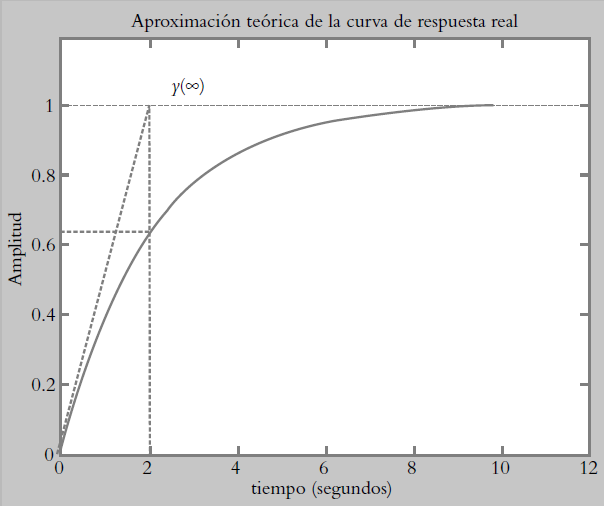
\includegraphics[width=0.625\linewidth]{metodo_const_tiempo_func_transf}
    \caption{Método de la constante de tiempo}
    \label{fig:metodoctetiempo}
\end{figure}

Obtenido esto, se procede a elaborar un sistema de primer orden mediante la siguiente expresión:

$$ G(s) = \frac{k}{\tau \cdot s + 1} $$

Donde $k$ representa la ganancia estática, que es el valor al que tiende la salida del sistema cuando la entrada es una señal constante y el tiempo tiende a infinito. En otras palabras, es el factor de escala entre la entrada y la salida en estado estacionario.

Para identificar la ganancia estática $k$, partimos de que en estado estacionario la salida alcanza un valor constante $y(\infty)$. Además, se considera que estimulamos al actuador con una señal escalón, denominada $u(\infty)$. La ganancia estática se puede calcular como:

$$ k=\frac{y(\infty)}{u(\infty)} $$

Para medir la respuesta del motor, primero conectamos mecánicamente el eje del motorreductor a medir junto con el eje de otro motor testigo, el cual esta conectado a un osciloscopio. Con esta experiencia buscamos estimular al motorreductor con una señal escalón unitario y que el motor testigo genere una tensión que se puede registrar en el osciloscopio. De este modo obtuvimos los valores de tensión generada en el motor testigo y podemos estimar la respuesta del motorreductor. En la Figura \ref{fig:exprespmotor} se muestra un diagrama de la experiencia.

\begin{figure}[H]
    \centering
    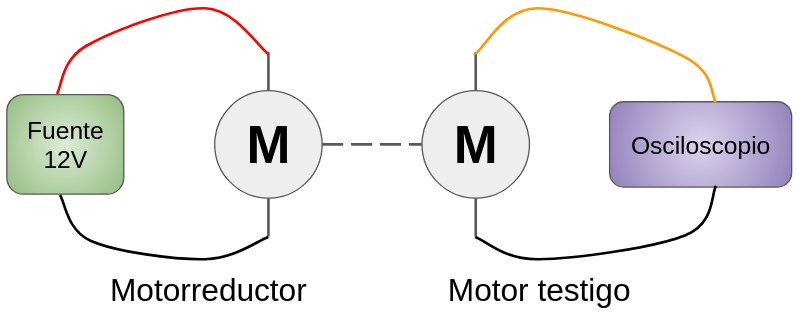
\includegraphics[width=0.55\linewidth]{experim_resp_motor}
    \caption{Experiencia para medición de RPM}
    \label{fig:exprespmotor}
\end{figure}

En el osciloscopio logramos obtener la gráfica que se muestra en la Figura \ref{fig:curvarespmotor}. En amarillo se representa la entrada escalón de 12V hacia el motor y en verde la tensión generada en el motor testigo.

\begin{figure}[H]
    \centering
    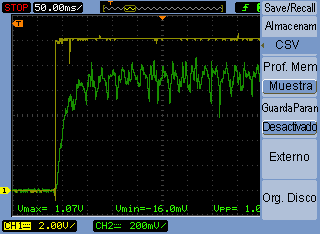
\includegraphics[width=0.525\linewidth]{curva_resp_motor_osciloscopio}
    \caption{Curva de respuesta del motorreductor}
    \label{fig:curvarespmotor}
\end{figure}

Luego procedimos a extraer los puntos de datos y suavizar la curva para facilitar el análisis. Esto lo hicimos mediante una media ponderada con un factor $\alpha = 0.2$, obtenido experimentalmente:

$$ S_{t} = \alpha \cdot Y_{t-1} + (1 - \alpha) \cdot Y_{t} $$

A partir de ello obtuvimos la gráfica de la Figura \ref{fig:curvarespmotorsuaviz}, donde en el eje horizontal están representados instantes de tiempo equivalentes a $10[ms]$ cada uno y en el eje vertical el voltaje (expresado en $[volts]$) sensado en el motor testigo.

Ahora bien, para linealizar el sistema podemos suponer que el valor de tensión generado en el motor testigo es proporcional a las revoluciones por minuto que gira su eje. Dado que en la iteración anterior se logró la implementación de un medidor de RPM, obtuvimos en este caso que el motorreductor conectado a 12V continuos produce 92 [RPM]. En este momento podemos calcular la ganancia estática $k$:

$$ k=\frac{y(\infty)}{u(\infty)}=\frac{92[RPM]}{12[V]}=7.66[RPM/V] $$

\begin{figure}[H]
    \centering
    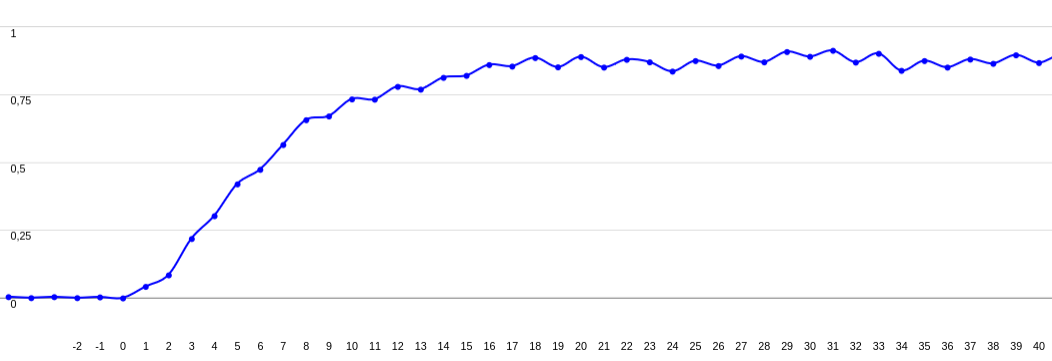
\includegraphics[width=1.0\linewidth]{resp_motor_suavizado}
    \caption{Curva de respuesta del motor suavizada}
    \label{fig:curvarespmotorsuaviz}
\end{figure}

Por otra parte, determinamos que $\tau=70[ms]$ por alcanzar en esa marca el valor de tensión $0,564[V]$, rondando el $63.2\%$ del valor en estado estacionario. Aplicando la expresión para obtener un sistema de primer orden obtenemos:

$$ G(s) = \frac{7.66}{0.07 \cdot s + 1} $$

% https://dademuchconnection.wordpress.com/2021/06/26/aproximacion-teorica-de-una-curva-de-respuesta-real/
% https://controlautomaticoeducacion.com/control-realimentado/ziegler-nichols-sintonia-de-control-pid/

\paragraph{Diseño del controlador} \mbox{} \vspace{8pt}

Es tarea del controlador intervenir para corregir las fluctuaciones que sufre el sistema. Por lo general los controladores PID basan su funcionamiento en 3 parámetros fundamentales, los cuales son $K_p$, $K_i$ y $K_d$; correspondiéndose con el factor de acción proporcional, integrativa y derivativa, respectivamente.

En nuestro caso, optamos por utilizar un PID aditivo por ser de sencilla implementación y por ser mas rápida la convergencia a los coeficientes óptimos. En la Figura \ref{fig:pidaditivo} se muestra un diagrama del mismo.

\begin{figure}[H]
    \centering
    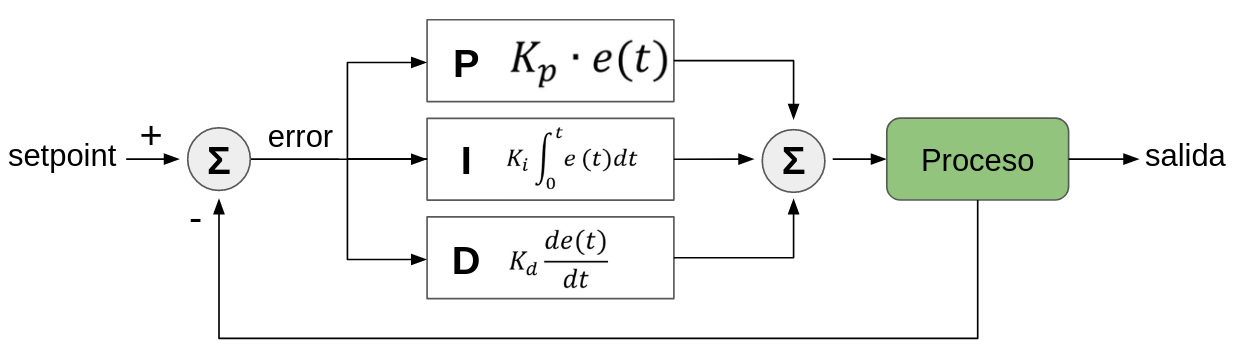
\includegraphics[width=1.0\linewidth]{images/pid_aditivo}
    \caption{PID aditivo}
    \label{fig:pidaditivo}
\end{figure}

\paragraph{Implementación} \mbox{} \vspace{8pt}

Cada uno de los cuatro motores del robot tiene su propio controlador PID, todos con coeficientes idénticos. Se implementan dentro del microcontrolador ESP32 haciendo uso de los puertos de salida PWM para controlar la velocidad y sentido de cada una de las ruedas. Además se utilizan los módulos contadores de pulsos asociados a los puertos GPIO donde se conecta cada encoder rotativo.

Como requerimiento, debe contar con tiempos de respuesta aceptables para que el sistema de control funcione adecuadamente, por lo que hicimos pruebas para descubrir el mejor $\Delta T$ de actualización del PID, en concordancia con el período de medición de RPM. Pudimos determinar que el controlador cumple con el requerimiento teniendo un periodo mínimo de $T=100[ms]$.

Por cada motor se tiene una estructura como la siguiente:

\begin{figure}[H]
    \centering
    \hspace*{-0.75cm}
    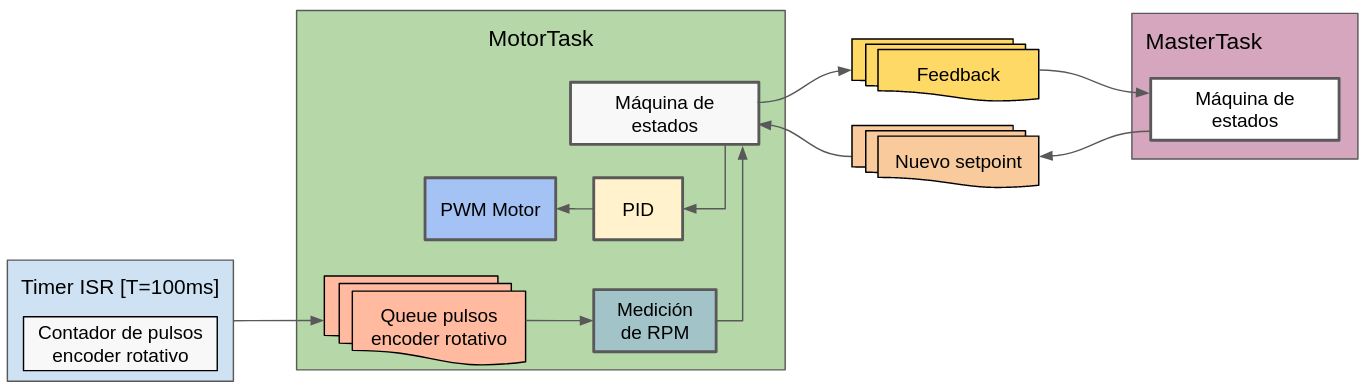
\includegraphics[width=1.1\linewidth]{images/diag_comp_esp32_pid_solo.png}
    \caption{Diagrama de componentes del firmware de la ESP32}
    \label{fig:diagcomponentesp32}
\end{figure}

En primer lugar, se tiene una interrupción periódica de $T=100[ms]$ donde se toman los valores de cada uno de los módulos contadores de pulso (PCNT) del microcontrolador, vinculados a los encoders rotativos de cada rueda. Existe una cola por cada MotorTask para recibir esta información desde la interrupción. Por otro lado, la tarea MasterTask cuenta con una cola (queue) única que comparte con todas las MotorTask para recibir el feedback de las mismas. Asimismo, cada tarea MotorTask tiene una cola que comparte con la tarea MasterTask, donde se envía un setpoint independiente a cada rueda.

Al ser el robot omnidireccional, si se establecen todas las ruedas a la misma velocidad y en sentidos determinados, es posible lograr que el robot de mueva a lo largo de un vector en linea recta sobre el plano. De este modo podemos llevar a cabo pruebas con las que encontramos los coeficientes del controlador.

A continuación, incurrimos en la utilización de la técnica de Ziegler-Nichols a lazo abierto y logramos obtener valores aproximados de $K_p$, $K_i$ y $K_d$. Introdujimos estos valores en el controlador y colocamos el robot en el suelo para realizar una serie de pruebas en línea recta. Con estos coeficientes no notamos un comportamiento óptimo, por lo que nos enfocamos en iterar sobre los valores y ajustar las constantes.

De este modo se realizaron iteraciones aumentando o disminuyendo cada uno de los coeficientes para buscar el punto óptimo de funcionamiento. Comenzamos con un valor de $K_p=10$ y un setpoint de $65[RPM]$, los demás coeficientes en cero. De este modo se fue aproximando el valor hasta lograr un arranque rápido pero sin demasiado sobrepaso. Una vez obtenido lo anterior, se procedió a ajustar $K_i$ observando cómo variaba el error acumulado al alcanzar las RPM deseadas. Para finalizar, se determinó el factor $K_d$ mediante observación de la respuesta del robot ante picos de perturbaciones.

Finalmente, obtenemos la siguiente estructura para el control de las 4 ruedas independientes del robot:

\begin{figure}[H]
    \centering
    \hspace*{-0.75cm}
    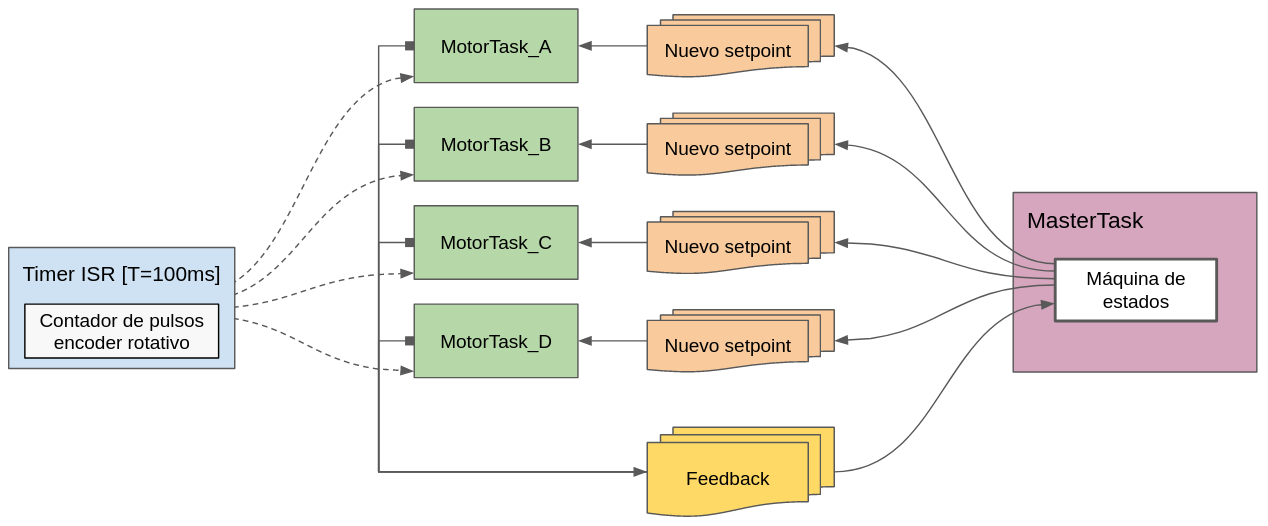
\includegraphics[width=1.05\linewidth]{images/diag_comp_esp32_pid_solo_todos_los_motores.png}
    \caption{Estructura de control de los motores}
    \label{fig:diagcommpesp32pidmotores}
\end{figure}

A continuación se detalla el funcionamiento de una de las tareas de los motores con la tarea principal. El proceso es similar para las demás MotorTask.

\begin{figure}[H]
    \centering
    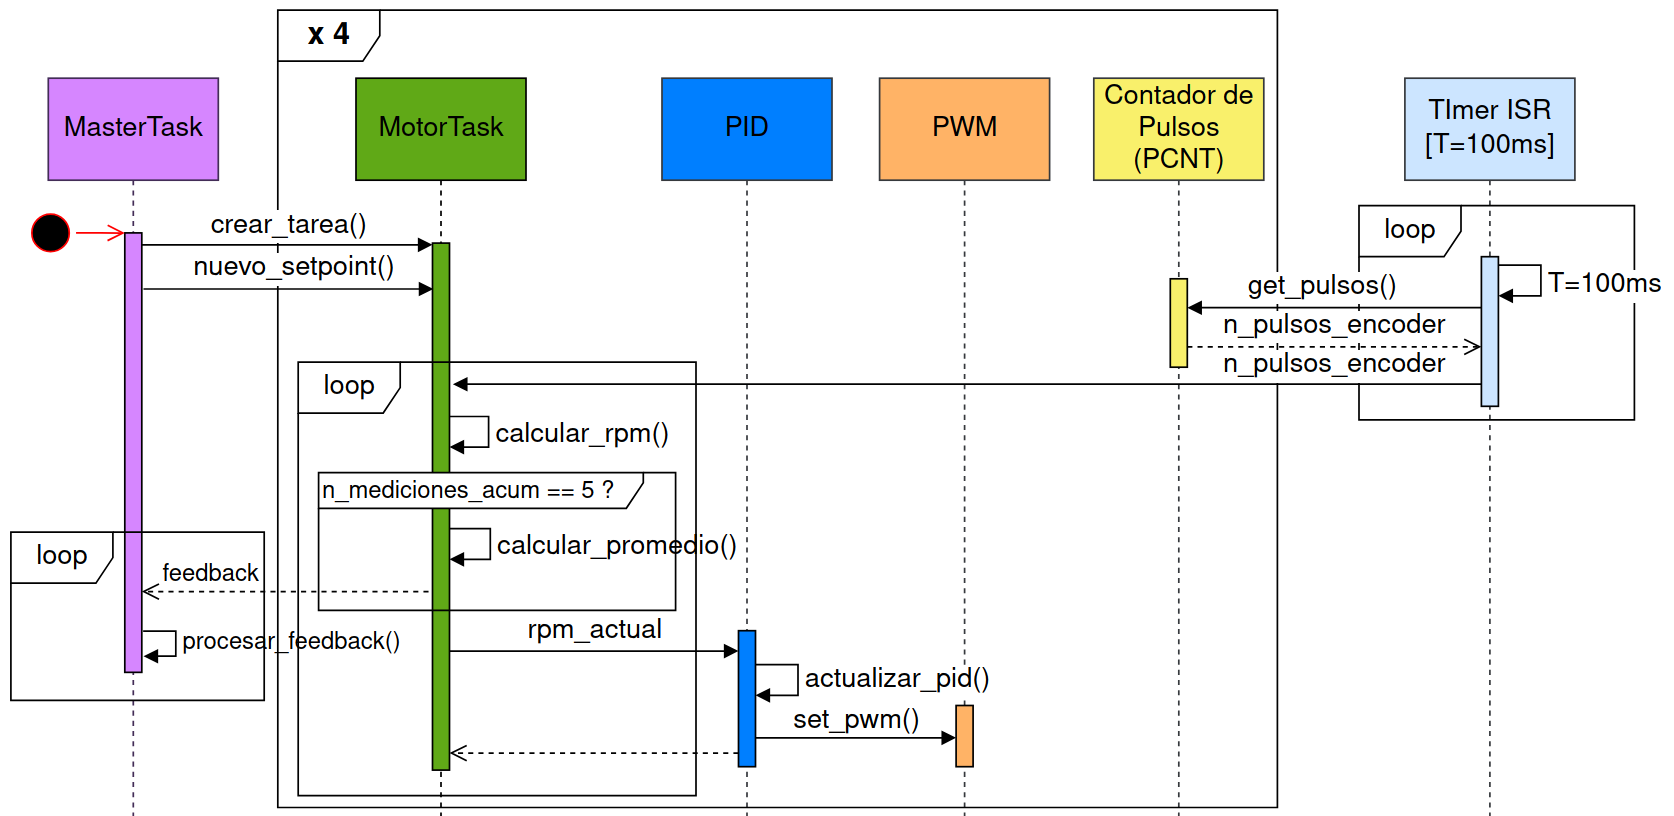
\includegraphics[width=1.1\linewidth]{images/diag_secuencia_pid_solo.png}
    \caption{Diagrama de secuencia de las tareas de control para los motores}
    \label{fig:diagsecuenciapidsolo}
\end{figure}


% fuentes de esta seccion 
% https://www.mdpi.com/2076-3417/12/5/2606
% https://tesis.ipn.mx/jspui/bitstream/123456789/18688/1/Sistema%20de%20control%20para%20el%20desplazamiento%20omnidireccional%20de%20un%20robot%20m%C3%B3vil.pdf


\subsubsection{Modelo cinemático}

La cinemática se define como la ciencia que estudia el movimiento de objetos sin tomar en cuenta sus inercias. Dentro de la misma se estudia la posición, la velocidad, la aceleración y todas las demás derivadas de alto orden de las variables de posición con respecto al tiempo.

Para lograr representar matemáticamente al robot se utilizan ecuaciones que relacionan las velocidades de las ruedas con la velocidad lineal y angular del robot en el plano. Estas ecuaciones se derivan de la disposición geométrica de las ruedas y las características de las ruedas omnidireccionales. Utilizando matrices de transformación, es posible describir cómo las velocidades de las ruedas se combinan para producir el movimiento deseado del robot. Para ello se definen dos elementos fundamentales, la ecuación cinemática directa y la ecuación cinemática inversa. \cite{tzafestas2013introduction}

En el contexto de un robot omnidireccional de 4 ruedas, la cinemática directa permite traducir un vector de movimiento lineal del robot en velocidades específicas para cada rueda independiente. Cada rueda se mueve independientemente y por su configuración, permite que el robot se pueda desplazar lateralmente, hacia adelante, hacia atrás, gire sobre su propio eje y realice trayectorias curvas. \cite{rijalusalamkinematics}

Es importante que tengamos en cuenta que para tener un sistema de control acotado y predecible, es necesario compensarlo de algún modo. En este caso debemos ser capaces de obtener el vector de movimiento del robot en base a las velocidades angulares medidas en las ruedas y así lograr detectar diferencias con el vector de movimiento deseado. Para ello nos resulta útil la cinemática inversa, que implica medir las velocidades angulares de cada una de las cuatro ruedas para obtener el vector de movimiento que el robot realiza. Esto es crucial para el control y navegación del robot dado que corrige las alteraciones de un entorno dinámico.

El desarrollo de estas ecuaciones implica calcular cómo las velocidades de cada rueda contribuyen al movimiento global del robot y cómo se deben ajustar estas velocidades para lograr una trayectoria específica. En otras palabras, estas ecuaciones toman en cuenta la disposición y orientación de las ruedas y cómo contribuyen al movimiento global del robot, aprovechando al máximo la capacidad omnidireccional del robot.

Una vez logrado un modelo cinemático que aproxime bien el sistema real, deberíamos poder establecer un vector de movimiento deseado y obtener la velocidad a la que se debe colocar cada rueda para poder transcurrirlo. No solo debería poder hacer movimientos rectos en cualquier dirección, sino que también sería capaz de hacer movimientos rotatorios con traslación sobre el plano, formando trayectorias elípticas. \cite{rijalusalamkinematics}

En nuestro caso se trata de un robot cuadrado con 1 rueda por cada lado cuya orientación respecto al robot es fija. Ademas de ello, se utilizan ruedas de tipo Omni-wheel, las cuales son similares a las ruedas Mecanum. Son ruedas que cuentan con pequeños discos (llamados rodillos) alrededor de la circunferencia perpendiculares a la dirección de giro. El efecto es que la rueda puede moverse con toda su fuerza, pero también se deslizará lateralmente con gran facilidad.

\begin{figure}[H]
    \centering
    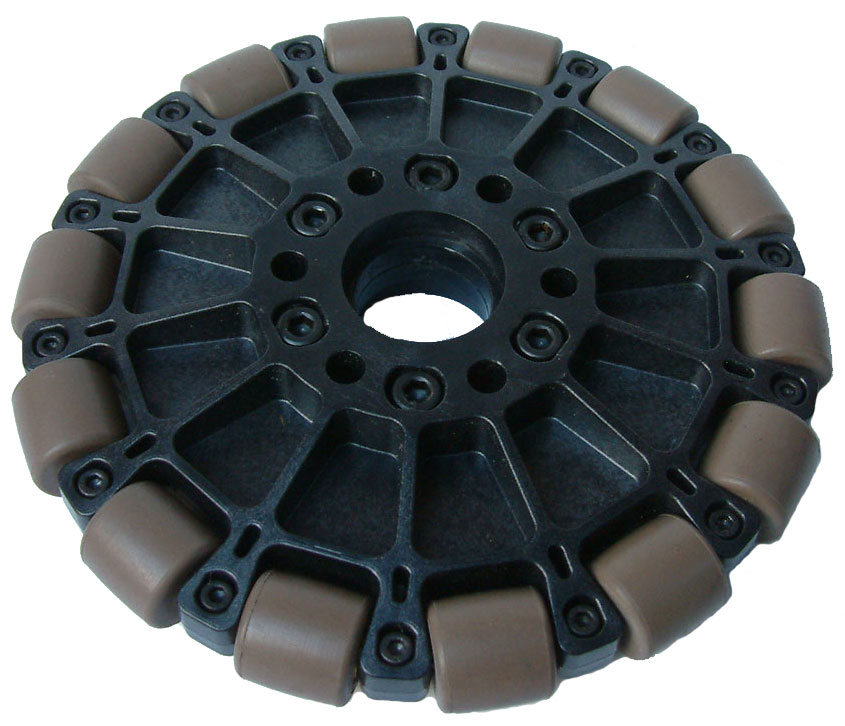
\includegraphics[width=0.3\linewidth]{omni-wheel-wikipedia}
    \caption{Rueda omnidireccional Omni-Wheel}
    \label{fig:ruedaomniwheel}
\end{figure}

Teniendo en cuenta lo anterior, para la construcción del modelo cinemático se consideran las siguientes limitaciones:

\begin{itemize}
    \item El robot se mueve sobre una superficie plana lisa.
    \item No existen elementos flexibles en la estructura del robot.
    \item El eje de direccionamiento de las ruedas siempre es perpendicular al suelo.
    \item No se consideran ningún tipo de fricciones contra el suelo.
\end{itemize}

\paragraph{Desarrollo} \mbox{} \vspace{8pt}

Al suponerse la rueda como un elemento rígido, se establece el principio de que las ruedas en contacto con el suelo se comportan como una articulación planar de tres grados de libertad, con lo que se propone el sistema de referencia descrito en la siguiente figura:

\begin{figure}[H]
    \centering
    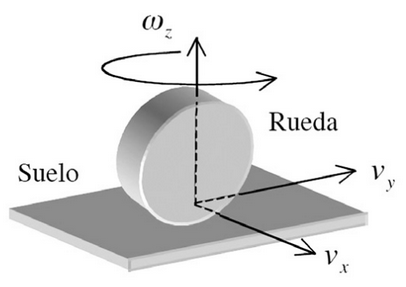
\includegraphics[width=0.4\linewidth]{rueda_modelo_cinematico}
    \caption{Vectores actuantes en una rueda}
    \label{fig:vectoresrueda}
\end{figure}

El eje $V_y$ determina el sentido normal de avance de la rueda, el eje $V_x$ indica los desplazamientos laterales y $\omega_z$ la velocidad rotacional que se produce cuando el vehículo realiza un giro.

Definimos al robot sobre el plano cartesiano, donde se establece el marco de referencia global representado por $oxy$ y el marco de referencia local del robot $o_rx_ry_r$, donde el marco de referencia local se encuentra alineado con el marco de referencia global.

\begin{figure}[H]
    \centering
    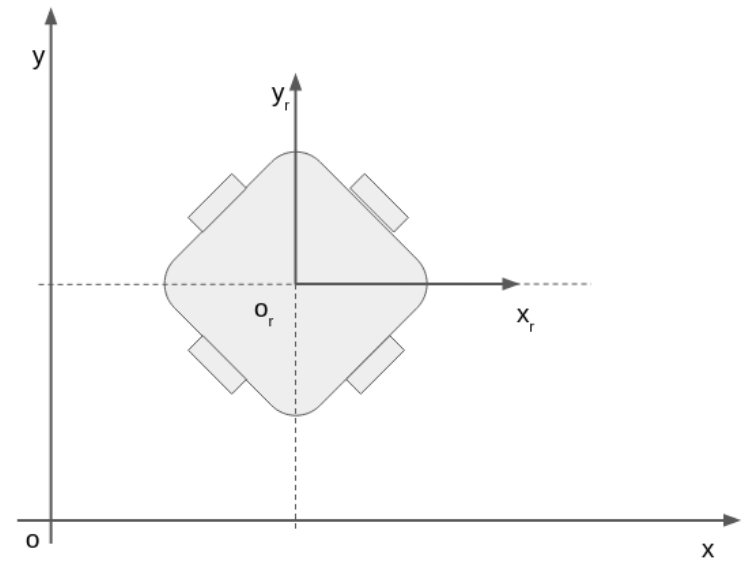
\includegraphics[width=0.6\linewidth]{robot_en_el_plano_mod_cinem}
    \caption{Marco de referencia del robot y del espacio}
    \label{fig:marcorefrobotenelplano}
\end{figure}

Además podemos representar el robot y la distribución de ruedas del siguiente modo:

\begin{figure}[H]
    \centering
    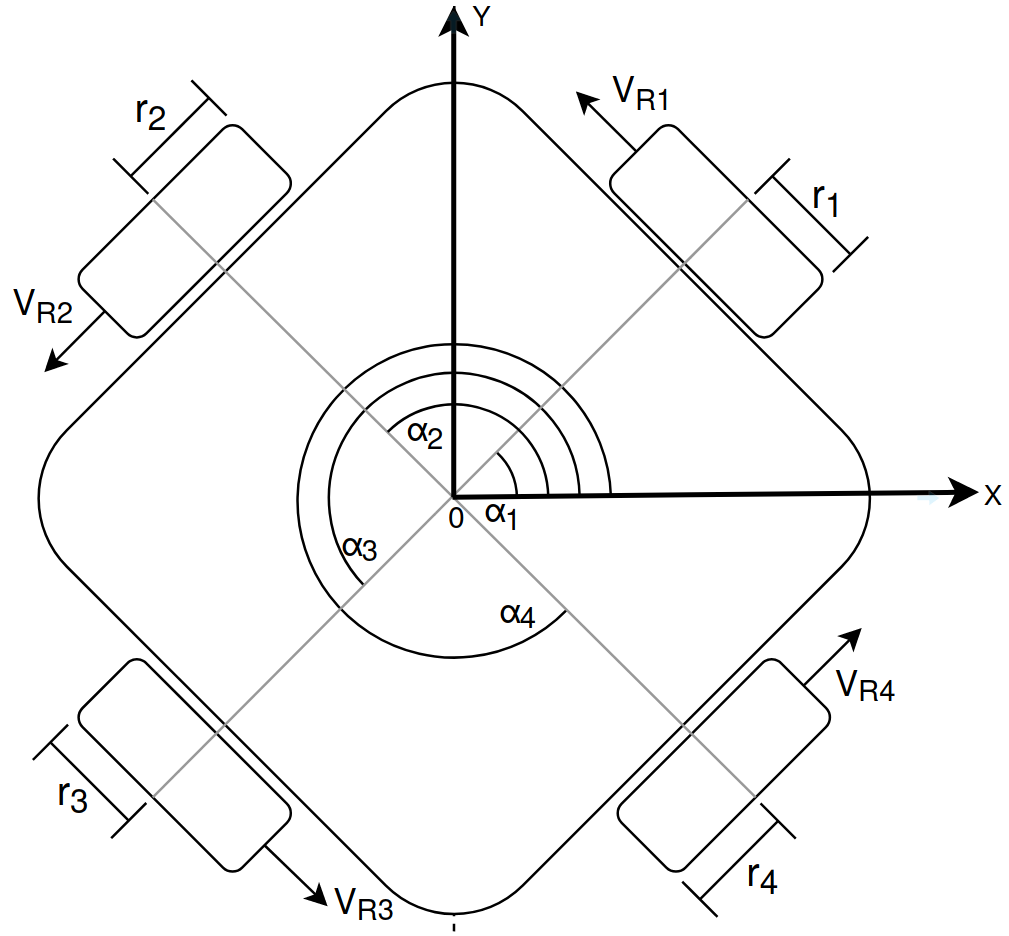
\includegraphics[width=0.6\linewidth]{images/modelo_cinematico_robot_ruedas.png}
    \caption{Descomposición de vectores del robot}
    \label{fig:vectoresrobotmodelocinem}
\end{figure}

Se establece que el angulo entre las ruedas y el cuerpo del robot es fijo y está dado por:

$$ \alpha_1 = \frac{\pi}{4} = 45^{\circ} $$
$$ \alpha_2 = \frac{3\pi}{4} = 135^{\circ} $$
$$ \alpha_3 = \frac{5\pi}{4} = 225^{\circ} $$
$$ \alpha_4 = \frac{7\pi}{4} = 315^{\circ} $$

%\newpage
\textbf{Cinemática Inversa} \mbox{} \vspace{8pt}

Para obtener el modelo cinemático, partimos del desarrollo de cómo afecta cada una de las ruedas al movimiento total del robot. Para ello comenzamos con la descripción del movimiento de un cuerpo rígido descrito en la Figura \ref{fig:movimientocuerporigido} \cite{islassistcontrolomni}.

$$ V_p = V_Q + W \times L $$

Utilizando el modelo de movimiento de cuerpo rígido, podemos expresar para el robot:

$$ V_{R1} = V_{01} + \omega_1 \times r_1 $$
$$ V_{R2} = V_{02} + \omega_2 \times r_2 $$
$$ V_{R3} = V_{03} + \omega_3 \times r_3 $$
$$ V_{R4} = V_{04} + \omega_4 \times r_4 $$

\begin{figure}[H]
    \centering
    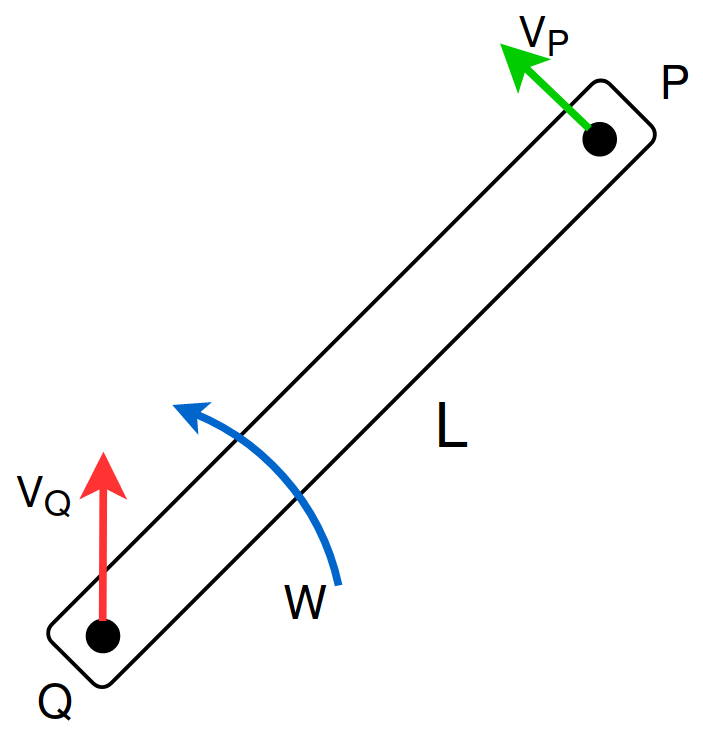
\includegraphics[width=0.3\linewidth]{images/movimiento_cuerpo_rigido.png}
    \caption{Movimiento de un cuerpo rígido}
    \label{fig:movimientocuerporigido}
\end{figure}

Se consideran $ V_{01}, V_{02}, V_{03}, V_{04} $ nulos dado que no existe deslizamiento entre las ruedas y el piso, además si todas las ruedas tienen el mismo radio, podemos expresar:

$$ V_{R1} = \omega_1 \times r $$
$$ V_{R2} = \omega_2 \times r $$
$$ V_{R3} = \omega_3 \times r $$
$$ V_{R4} = \omega_4 \times r $$

Ahora, podemos analizar el marco de referencia de la rueda respecto al marco de referencia del robot. Para ello:

\begin{figure}[H]
    \centering
    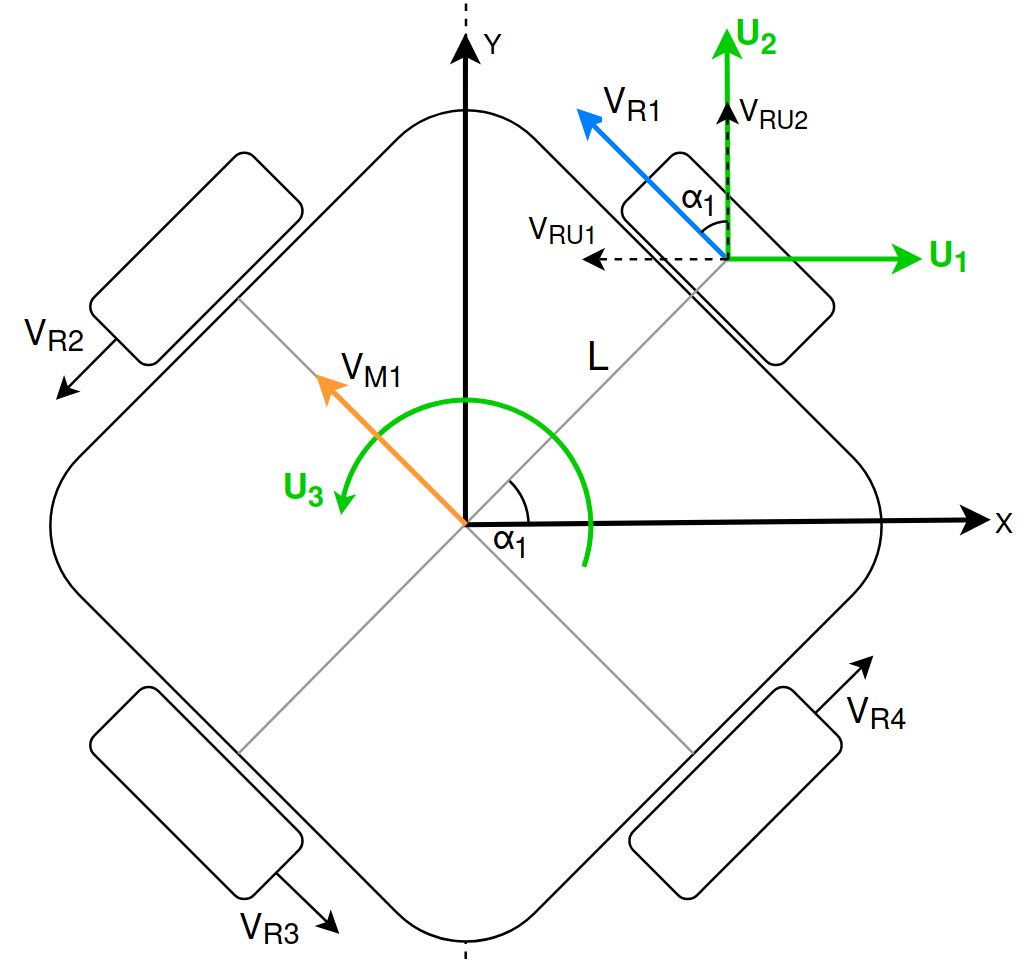
\includegraphics[width=0.6\linewidth]{images/modelo_cinematico_robot_vector.png}
    \caption{Vectores del robot en el marco de referencia local}
    \label{fig:robotmarcoreflocal}
\end{figure}

Se plantea el caso para una de las ruedas. Para obtener el vector $V_{R1}$ en base al marco de referencia denotado por $U_1$, $U_2$ y $U_3$, podemos hacer:

$$ V_{R1} = V_{M1} + U_3 \times L $$

De modo que podemos expresar $V_{M1}$ en función de $U_1$ y $U_2$:

$$ V_{M1} = V_{RU_1} + V_{RU_2} $$
$$ V_{M1} = -U_1 \cdot sen(\alpha_1) + U_2 \cdot cos(\alpha_1) $$

Obteniendo finalmente que:

$$ V_{R1} = -U_1 \cdot sen(\alpha_1) + U_2 \cdot cos(\alpha_1) + U_3 \times L $$

Al realizar el mismo procedimiento para las demás ruedas obtenemos:

$$ V_{R1} = -U_1 \cdot sen(\alpha_1) + U_2 \cdot cos(\alpha_1) + U_3 \times L $$
$$ V_{R2} = -U_1 \cdot sen(\alpha_1) + U_2 \cdot cos(\alpha_1) + U_3 \times L $$
$$ V_{R4} = -U_1 \cdot sen(\alpha_1) + U_2 \cdot cos(\alpha_1) + U_3 \times L $$
$$ V_{R3} = -U_1 \cdot sen(\alpha_1) + U_2 \cdot cos(\alpha_1) + U_3 \times L $$

Ahora bien, si $U_1$, $U_2$ y $U_3$ están alineados respecto al marco de referencia global $0XY$, podemos expresar:

$$ \begin{bmatrix} U_1 \\ U_2 \\ U_3 \end{bmatrix} = \begin{bmatrix} V_x \\ V_y \\ V_\theta \end{bmatrix} $$

Entonces ahora podemos hacer la siguiente igualdad con lo obtenido:

$$ \omega_1 \times r = -V_x \cdot sen(\alpha_1) + V_y \cdot cos(\alpha_1) + V_\theta \times L $$
$$ \omega_2 \times r = -V_x \cdot sen(\alpha_2) + V_y \cdot cos(\alpha_2) + V_\theta \times L $$
$$ \omega_3 \times r = -V_x \cdot sen(\alpha_3) + V_y \cdot cos(\alpha_3) + V_\theta \times L $$
$$ \omega_4 \times r = -V_x \cdot sen(\alpha_4) + V_y \cdot cos(\alpha_4) + V_\theta \times L $$

Originalmente partimos de que necesitamos una matriz de conversión de modo que podamos obtener las velocidades de las ruedas en base a un vector dado, donde la entrada es $V_x, V_y$ expresadas en $[m/seg]$ y $V_\theta$ expresada en $[RPM]$. Por otra parte, la salida $\omega_n$ se determina en $[rad/seg]$:

$$ \begin{bmatrix} w_1 \\ w_2 \\ w_3 \\ w_4 \\ \end{bmatrix} = IK \cdot \begin{bmatrix} V_x \\ V_y \\ V_\theta \\ \end{bmatrix} $$

Con las expresiones anteriores, obtenemos que la matriz cinemática inversa se puede expresar como:

$$ IK = 
    \frac{1}{r}
    \cdot
    \begin{bmatrix}
        {-sen(\alpha_1)} & {cos(\alpha_1)} & L \\
        {-sen(\alpha_2)} & {cos(\alpha_2)} & L \\
        {-sen(\alpha_3)} & {cos(\alpha_3)} & L \\
        {-sen(\alpha_4)} & {cos(\alpha_4)} & L \\
    \end{bmatrix} $$

De modo que podemos expresar la ecuación para obtener las velocidades de las ruedas expresadas en $[rad/seg]$ como se muestra debajo.

$$ \begin{bmatrix} w_1 \\ w_2 \\ w_3 \\ w_4 \\ \end{bmatrix} = \frac{1}{r} \cdot \begin{bmatrix}
    {-sen(\frac{\pi}{4})} & {cos( \frac{\pi}{4})} & L \\
    {-sen(\frac{3\pi}{4})} & {cos(\frac{3\pi}{4})} & L \\
    {-sen(\frac{5\pi}{4})} & {cos(\frac{5\pi}{4})} & L \\
    {-sen(\frac{7\pi}{4})} & {cos(\frac{7\pi}{4})} & L \\
\end{bmatrix} \cdot
\begin{bmatrix} V_x \\ V_y \\ V_\theta \\ \end{bmatrix} $$

Dado que las MotorTask de cada una de las ruedas recibe el setpoint en $[RPM]$, debemos hacer una conversión a esa unidad. Por lo que planteamos una matriz que convierta los valores de las dos primeras columnas de la matriz cinemática, que son los coeficientes que nos interesa convertir a $[RPM]$, dado que los de la última columna ya están expresados en esa unidad.

$$ \begin{bmatrix} w_1 \\ w_2 \\ w_3 \\ w_4 \\ \end{bmatrix} =
    \frac{1}{r}
    \cdot
    \begin{bmatrix}
        {-sen(\frac{\pi}{4})} & {cos( \frac{\pi}{4})} & L \\
        {-sen(\frac{3\pi}{4})} & {cos(\frac{3\pi}{4})} & L \\
        {-sen(\frac{5\pi}{4})} & {cos(\frac{5\pi}{4})} & L \\
        {-sen(\frac{7\pi}{4})} & {cos(\frac{7\pi}{4})} & L \\
    \end{bmatrix}
    \cdot
    \begin{bmatrix}
        {\frac{60}{2 \pi}} & {0} & {0} \\
        {0} & {\frac{60}{2 \pi}} & {0} \\
        {0} & {0} & {1}                \\
    \end{bmatrix}
    \cdot
    \begin{bmatrix} V_x \\ V_y \\ V_\theta \\ \end{bmatrix} $$


\textbf{Cinemática Directa} \mbox{} \vspace{8pt}

Para lograr el control del robot sobre el plano es necesario hacer una comparación entre el vector de movimiento deseado y un vector de movimiento inferido en base a la medición de la velocidad de las ruedas, de modo que se cierra el lazo de control. El error existente entre el vector real y el deseado es debido a que los motores no establecen las RPM inmediatamente por cuestiones de inercia e imperfecciones en el terreno.

Para obtener el vector de velocidad lineal real que efectivamente realiza el robot, hacemos uso de las mediciones de velocidad angular en cada rueda y se ingresan a la ecuación cinemática directa. Esta matriz se obtiene a partir de la pseudoinversa de la matriz cinemática inversa. \cite{islassistcontrolomni}

De modo que, en primer lugar obtenemos la matriz de conversión que nos permite obtener el vector lineal en base a las velocidades de las ruedas expresadas en $[rad/seg]$:

$$ \begin{bmatrix} V_x \\ V_y \\ V_\theta \\ \end{bmatrix} = DK \cdot \begin{bmatrix} w_1 \\ w_2 \\ w_3 \\ w_4 \\ \end{bmatrix} $$

Luego, al realizar la pseudoinversa de la matriz $IK$:

$$  DK = 
    r
    \cdot 
    \begin{bmatrix}
        {\frac{-sen(\alpha_1)}{2}} & {\frac{-sen(\alpha_2)}{2}} & {\frac{-sen(\alpha_3)}{2}} & {\frac{-sen(\alpha_4)}{2}} \\
        {\frac{cos(\alpha_1)}{2}}  & {\frac{cos(\alpha_2)}{2}}  & {\frac{cos(\alpha_3)}{2}}  & {\frac{cos(\alpha_4)}{2}}  \\
        {\frac{1}{4L}}  & {\frac{1}{4L}}  & {\frac{1}{4L}}  & {\frac{1}{4L}}  \\
    \end{bmatrix} $$

Por lo que obtenemos la siguiente expresión para obtener el vector de movimiento del robot dependiendo de las velocidades de las ruedas:

$$ \begin{bmatrix} V_x \\ V_y \\ V_\theta \\ \end{bmatrix} = 
    r
    \cdot 
    \begin{bmatrix}
        {\frac{-sen(\alpha_1)}{2}} & {\frac{-sen(\alpha_2)}{2}} & {\frac{-sen(\alpha_3)}{2}} & {\frac{-sen(\alpha_4)}{2}} \\
        {\frac{cos(\alpha_1)}{2}}  & {\frac{cos(\alpha_2)}{2}}  & {\frac{cos(\alpha_3)}{2}}  & {\frac{cos(\alpha_4)}{2}}  \\
        {\frac{1}{4L}}  & {\frac{1}{4L}}  & {\frac{1}{4L}}  & {\frac{1}{4L}}  \\
    \end{bmatrix}
    \cdot
    \begin{bmatrix} w_1 \\ w_2 \\ w_3 \\ w_4 \\ \end{bmatrix} $$

Esta expresión toma las velocidades angulares de las ruedas en $[rad/seg]$, por lo que necesitamos convertir la entrada para que pueda ser $[RPM]$. Para ello planteamos una matriz que solo convierta los valores de las dos primeras filas, que son los coeficientes que nos interesa convertir a $[RPM]$, dado que los de la última fila ya están expresados en esa unidad.

$$ \begin{bmatrix} V_x \\ V_y \\ V_\theta \\ \end{bmatrix} = 
    r
    \cdot 
    \begin{bmatrix}
        {\frac{2\pi}{60}} & {0} & {0}  \\
        {0} & {\frac{2\pi}{60}} & {0} \\
        {0} & {0} & {1} \\
    \end{bmatrix}
    \cdot
    \begin{bmatrix}
        {\frac{-sen(\alpha_1)}{2}} & {\frac{-sen(\alpha_2)}{2}} & {\frac{-sen(\alpha_3)}{2}} & {\frac{-sen(\alpha_4)}{2}} \\
        {\frac{cos(\alpha_1)}{2}}  & {\frac{cos(\alpha_2)}{2}}  & {\frac{cos(\alpha_3)}{2}}  & {\frac{cos(\alpha_4)}{2}}  \\
        {\frac{1}{4L}}  & {\frac{1}{4L}}  & {\frac{1}{4L}}  & {\frac{1}{4L}}  \\
    \end{bmatrix}
    \cdot
    \begin{bmatrix} w_1 \\ w_2 \\ w_3 \\ w_4 \\ \end{bmatrix} $$


\paragraph{Implementación} \mbox{} \vspace{8pt}

Para la implementación se propuso que el modelo cinemático sea contenido dentro de la MasterTask dado que es quien recibe el feedback de todas las tareas MotorTask y conoce el estado actual de cada uno de los motores. Un diagrama de secuencia se detalla más adelante en este capítulo.

\begin{figure}[H]
    \centering
    \hspace*{-0.75cm}
    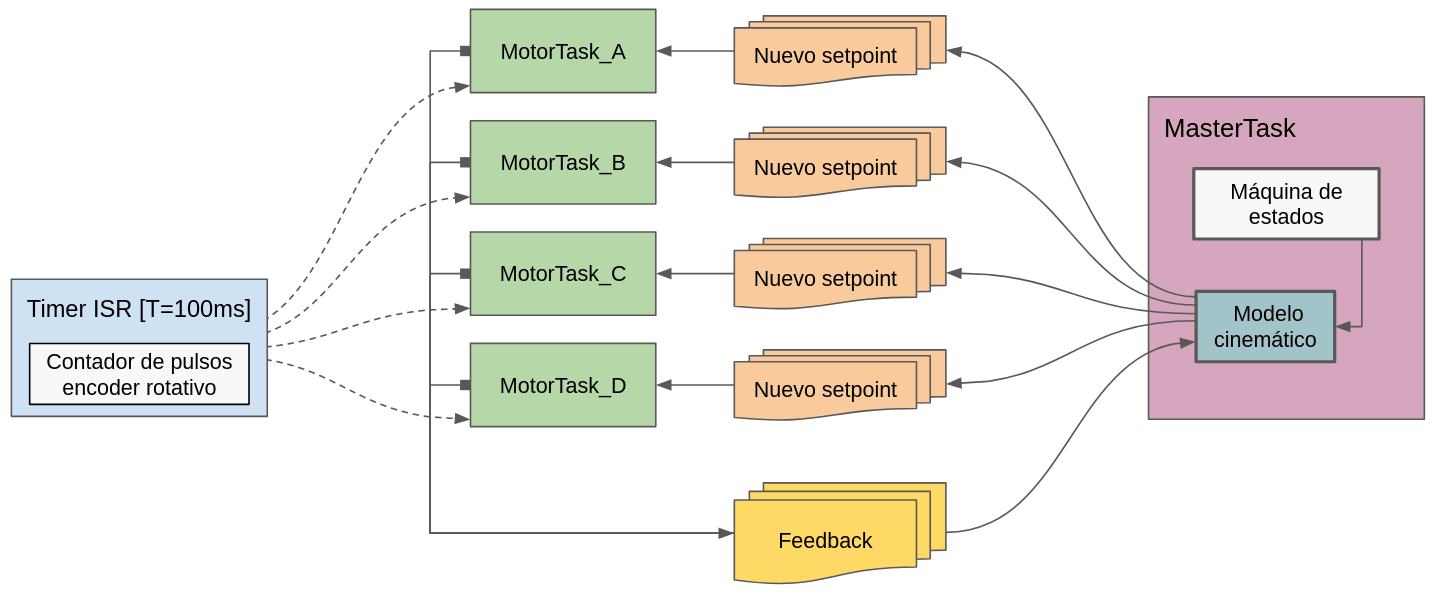
\includegraphics[width=1.1\linewidth]{images/diag_comp_esp32_modelo_cinem.png}
    \caption{Estructura de control de los motores con el Modelo Cinemático}
    \label{fig:diagcomponentesp32modelocinem}
\end{figure}


\subsubsection{Odometría}

La odometría es el proceso mediante el cual un robot estima su posición y orientación en el espacio a lo largo del tiempo. Esta técnica se utiliza para obtener una aproximación de la trayectoria recorrida por el robot, a partir de los desplazamientos medidos en sus ruedas o actuadores, generalmente utilizando sensores como pueden ser encoders rotativos o lineales.

Dado que necesitamos estimar la posición y orientación del robot en el espacio a lo largo del tiempo, nos podemos basar en las lecturas de los sensores de las ruedas. Para inferir la distancia recorrida podemos medir las velocidades angulares o la distancia recorrida de cada una de las cuatro ruedas en simultáneo. Estos datos se obtienen a partir de los encoders rotativos instalados en las ruedas.

Se probaron distintas alternativas para el proceso de odometría. Primeramente se probó de modo que cada rueda recibe la distancia que debe recorrer el robot y de modo independiente mide cuanto recorre para determinar si debe detenerse o no. Concluimos que esta técnica tiene algunos problemas porque no considera a nivel global el movimiento del robot y como influyen las perturbaciones de las demás ruedas sobre una de ellas. Es por ello que optamos por hacer uso del modelo cinemático para realizar la odometría. Este método no excluye de errores al proceso, pero tiene en consideración todas las ruedas al momento de determinar la distancia recorrida por el robot dada la sumatoria de la acción de todas ellas. \cite{palacinodometry}

La odometría se basa en el uso del modelo cinemático para convertir estas velocidades angulares en velocidades lineales y angulares del robot en el plano, es decir, obtener un vector de movimiento en base a las mediciones. Para ello, el primer paso en el proceso es utilizar las ecuaciones del modelo cinemático directo para calcular las velocidades lineales y angulares en el instante $t$ a partir de las velocidades de las ruedas: ($V_xt$, $V_yt$, $V_\theta t$). Posteriormente se pueden integrar estas velocidades a lo largo del tiempo para estimar la posición ($x, y$) y la orientación ($\theta$) del robot. La integración se realiza mediante métodos numéricos, típicamente utilizando un enfoque de integración discreta, como el método de Euler. Por lo que en cada instante de tiempo que se toma una medición, se actualiza la posición y orientación del robot utilizando las siguientes ecuaciones, donde ($\Delta$t) es el intervalo de tiempo entre dos mediciones consecutivas:

$$ x_{t+1} = x_t + V_xt \cdot \Delta t $$

$$ y_{t+1} = y_t + V_yt \cdot \Delta t $$

$$ \theta_{t+1} = \theta_t + V_\theta t \cdot \Delta t $$

Es importante considerar que la odometría realizada para ruedas puede acumular errores debido a factores como el deslizamiento de las ruedas, inexactitudes en las mediciones de los encoders o imprecisiones en los cálculos. Por lo tanto, es común combinar la odometría con otros métodos de localización, como el uso de sensores adicionales (LIDAR, cámaras, etc.) y técnicas de fusión de datos (como los filtros de Kalman), para mejorar la precisión y robustez de la estimación de la posición del robot.

Para la realización de las pruebas colocamos marcas en el piso a 1 metro de distancia entre sí y realizamos iteraciones para verificar que la odometría opera dentro de los rangos de precisión establecidos.


\subsubsection{Envío y recepción de comandos}

Se implementó un sistema de comunicación basado en el protocolo MQTT (Message Queuing Telemetry Transport) para enviar y recibir informacion del robot. Se envían vectores a recorrer con una estructura de datos a modo de tupla de valores que representa la distancia a recorrer, las velocidades lineales y angulares del robot: $distancia [m]$, $V_x [m/seg]$, $V_y [m/seg]$ y $V_\theta [RPM]$.

Además, el robot es capaz de enviar información por medio de MQTT sobre la odometría y el estado en tiempo real. Esto resulta útil dado que posibilita monitorear el estado del robot y realizar ajustes si es necesario.

Por un lado, las velocidades $V_x$ y $V_y$ determinan un sentido de movimiento en linea recta sobre el plano. Por otro lado, $V_\theta$ controla la rotación del robot sobre su propio eje, permitiéndole girar en el plano horizontal.

Cuando se envía una tupla de valores de velocidad mediante MQTT, el robot calcula la velocidad para cada rueda usando el modelo cinemático y establece los motores a la velocidad estipulada, luego se detiene cumplida la distancia recorrida. En la Figura \ref{fig:diagcomponentesp32conmodelocinem} se muestra un diagrama de secuencia con los componentes integrados hasta el momento.

\begin{figure}[htb]
    \centering
    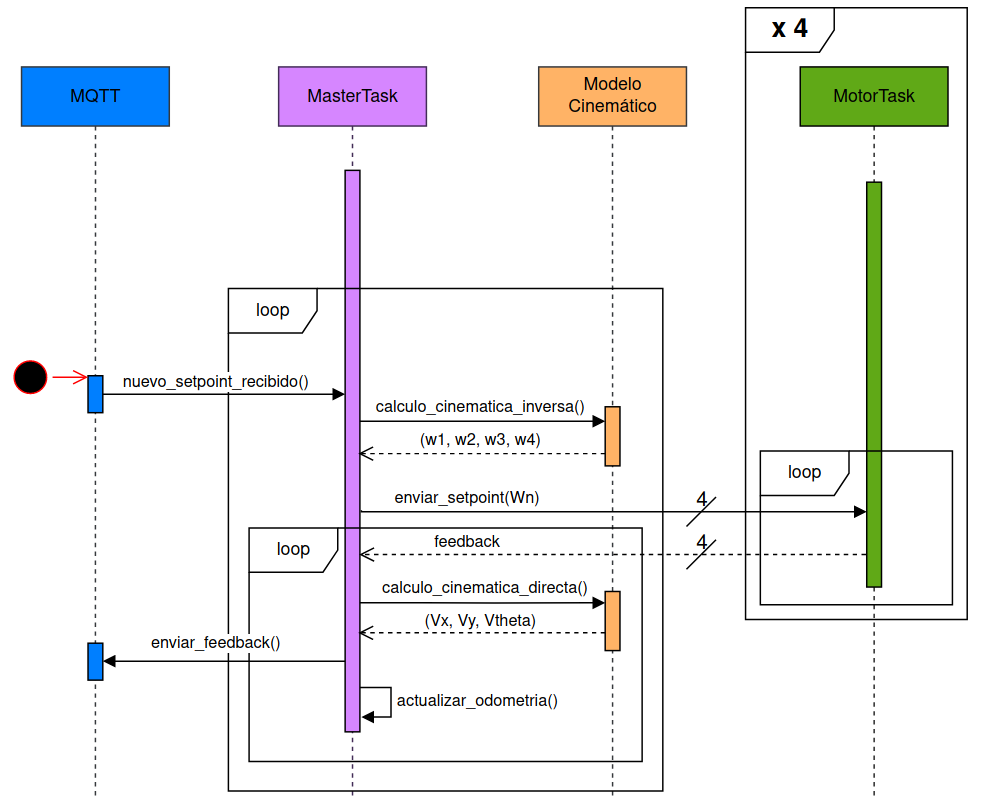
\includegraphics[width=1\linewidth]{images/diag_secuencia_full_modelo_cinematico.png}
    \caption{Diagrama de secuencia de la ESP32 con el Modelo Cinemático}
    \label{fig:diagcomponentesp32conmodelocinem}
\end{figure}


\subsubsection{Campo de pruebas}

En cualquier estudio experimental, es vital controlar todas las variables posibles para aislar el efecto de las variables independientes. La superficie sobre la que se desplaza el robot puede influir significativamente en su comportamiento, ya que las irregularidades de la misma pueden inducir deslizamientos o atascos.

La elección de una superficie determinada, consistente y constante en cada experimento es crucial para asegurar la fiabilidad de los resultados obtenidos, al proporcionar un entorno controlado. Mantener una superficie constante permite replicar las condiciones experimentales y comparar resultados de manera precisa y predecible. Si la superficie varía, se introducen variables adicionales que pueden afectar el desempeño del robot, dificultando la comparación entre experimentos.

En primera instancia, la superficie sobre la cual comenzamos las pruebas del prototipo fue el suelo del Laboratorio. En los sucesivos experimentos notamos cierta inconsistencia entre cada iteración, manteniendo los parámetros de funcionamiento constantes. En búsqueda de mejorar la consistencia entre los experimentos, hicimos algunas pruebas sobre un tablón de madera lisa y notamos que la mejoría es sustancial. En consecuencia, se dispone de una superficie de madera sobre la cual realizamos las subsiguientes pruebas.


\subsection{Testing y pruebas}

% https://en.wikibooks.org/wiki/LaTeX/Tables

\begin{testtableformat}
    \hline \rowcolor{test_header_color}
        Test ID             & TC\_01\_00 \\
    \hline
        Tipo de test        & Test unitario \\
    \hline
        Objeto de prueba    & Comunicación inalámbrica \\
    \hline
        Requerimiento       & RF6 \\
    \hline
        Nombre              & Comunicación inalámbrica para monitoreo y envío de comandos por MQTT \\
    \hline
        Descripción         & Verificar que los comandos son recibidos correctamente en el robot y que el robot envía información de estado en el formato correcto \\
    \hline
        Precondición        & PRECOND\_A \\
    \hline
        Pasos del test      & \begin{enumerate}
                                \item Enviar un nuevo setpoint con parámetros de distancia [50cm $\sim$ 200cm] y velocidad $\pm$[0.25m/seg $\sim$ 0.75m/seg]
                                \item Verificar que el robot recibe el comando correctamente y que envía reportes
                                \item Repetir desde el paso 1) con diferentes valores
                            \end{enumerate} \\
    \hline
        Resultado esperado  & El robot recibe e interpreta los comandos, al mismo tiempo que reporta información sobre su estado periódicamente \\
    \hline
        Resultado obtenido  & El robot realiza el comportamiento esperado, envía, recibe e interpreta comandos \\
    \hline
        Observaciones       & - \\
    \hline
\end{testtableformat}


\begin{testtableformat}
    \hline \rowcolor{test_header_color}
        Test ID             & TC\_01\_01 \\
    \hline
        Tipo de test        & Test unitario \\
    \hline
        Objeto de prueba    & PWM - Medidor de RPM \\
    \hline
        Requerimiento       & RF1 - RF5 \\
    \hline
        Nombre              & Medidor de RPM \\
    \hline
        Descripción         & Comprobar que al establecer el motor a determinada velocidad ésta se corresponda con la medición obtenida por el medidor de RPM \\
    \hline
        Precondición        & PRECOND\_A \\
    \hline
        Pasos del test      & \begin{enumerate}
                                \item Enviar un valor de PWM al controlador del motor entre [0 $\sim$ 1023]
                                \item Verificar que el motor se establece a la velocidad deseada y que el medidor de RPM informa el valor correcto
                                \item Repetir desde el paso 1) con diferentes valores
                            \end{enumerate} \\
    \hline
        Resultado esperado  & Se obtiene el valor correcto de RPM medido en cada iteración \\
    \hline
        Resultado obtenido  & En todas las iteraciones las mediciones reportan una velocidad cercana a la establecida \\
    \hline
        Observaciones       & La velocidad máxima que podemos obtener del motor sin carga son 92 RPM (PWM = 1023) y el motor comienza a girar continuamente cuando las RPM se establecen en una velocidad mínima de 55 RPM (PWM $\cong$ 420) \\
    \hline
\end{testtableformat}


\begin{testtableformat}
    \hline \rowcolor{test_header_color}
        Test ID             & TC\_01\_02 \\
    \hline
        Tipo de test        & Test de integración \\
    \hline
        Objeto de prueba    & PID - PWM - Medidor de RPM \\
    \hline
        Requerimiento       & RF1 - RF5 \\
    \hline
        Nombre              & PID sin carga \\
    \hline
        Descripción         & Verificar que el PID establece correctamente la velocidad de la rueda al recibir el setpoint en RPM sin carga vinculada a la rueda \\
    \hline
        Precondición        & PRECOND\_A \\
    \hline
        Pasos del test      & \begin{enumerate}
                                \item Enviar un valor de RPM al controlador PID del motor entre [0 $\sim$ 92] RPM
                                \item Verificar que el motor se establece a las RPM deseadas y que el medidor de RPM informa el valor correcto
                                \item Repetir desde el paso 1) con diferentes valores
                            \end{enumerate} \\
    \hline
        Resultado esperado  & Se obtiene el valor de RPM correcta en cada iteración \\
    \hline
        Resultado obtenido  & En todas las iteraciones se obtuvo que la rueda gira a una velocidad cercana a la establecida \\
    \hline
        Observaciones       & La velocidad máxima que podemos obtener del motor sin carga son 92 RPM y el motor comienza a girar continuamente cuando las RPM se establecen en una velocidad mínima de 55 RPM \\
    \hline
\end{testtableformat}


\begin{testtableformat}
    \hline \rowcolor{test_header_color}
        Test ID             & TC\_01\_03 \\
    \hline
        Tipo de test        & Test de integración \\
    \hline
        Objeto de prueba    & PID - PWM - Medidor de RPM \\
    \hline
        Requerimiento       & RF1 - RF5 \\
    \hline
        Nombre              & PID con carga \\
    \hline
        Descripción         & Verificar que el PID establece correctamente la velocidad de la rueda al recibir el setpoint en RPM con una carga aproximadamente igual al peso del robot \\
    \hline
        Precondición        & PRECOND\_A \\
    \hline
        Pasos del test      & \begin{enumerate}
                                \item Enviar un valor de RPM al controlador PID del motor entre [0 $\sim$ 92] RPM
                                \item Verificar que el motor se establece a las RPM deseadas y que el medidor de RPM informa el valor correcto
                                \item Repetir desde el paso 1) con diferentes valores
                            \end{enumerate} \\
    \hline
        Resultado esperado  & Se obtiene el valor de RPM correcta en cada iteración \\
    \hline
        Resultado obtenido  & En todas las iteraciones se obtuvo que la rueda gira a una velocidad cercana a la establecida \\
    \hline
        Observaciones       & La velocidad máxima que podemos obtener del motor con una carga presente son 88 RPM y el motor comienza a girar continuamente cuando las RPM se establecen en una velocidad mínima de 63 RPM \\
    \hline
\end{testtableformat}


\begin{testtableformat}
    \hline \rowcolor{test_header_color}
        Test ID             & TC\_01\_04 \\
    \hline
        Tipo de test        & Test unitario \\
    \hline
        Objeto de prueba    & Modelo Cinemático \\
    \hline
        Requerimiento       & RF2 - RF4 \\
    \hline
        Nombre              & Modelo Cinemático en línea recta \\
    \hline
        Descripción         & Comprobar que el Modelo Cinemático calcula adecuadamente las velocidades de las ruedas según un setpoint en línea recta \\
    \hline
        Precondición        & PRECOND\_B \\
    \hline
        Pasos del test      & \begin{enumerate}
                                \item Enviar al Modelo Cinemático un vector de velocidad en linea recta con valores entre $\pm$[0.25m/seg $\sim$ 0.75m/seg]
                                \item Colocar cada una de las ruedas a la velocidad calculada por el Modelo Cinemático y verificar que el robot se mueve a lo largo del vector definido
                                \item Repetir desde el paso 1) con diferentes valores
                            \end{enumerate} \\
    \hline
        Resultado esperado  & El robot se mueve en línea recta en la dirección del vector dado por $V_x$ y $V_y$ \\
    \hline
        Resultado obtenido  & Se observa que el robot realiza el comportamiento esperado \\
    \hline
        Observaciones       & - \\
    \hline
\end{testtableformat}


\begin{testtableformat}
    \hline \rowcolor{test_header_color}
        Test ID             & TC\_01\_05 \\
    \hline
        Tipo de test        & Test unitario \\
    \hline
        Objeto de prueba    & Modelo Cinemático \\
    \hline
        Requerimiento       & RF2 - RF4 \\
    \hline
        Nombre              & Modelo Cinemático en trayectorias curvas \\
    \hline
        Descripción         & Comprobar que el Modelo Cinemático calcula adecuadamente las velocidades de las ruedas según un setpoint con velocidad rotacional distinta de cero \\
    \hline
        Precondición        & PRECOND\_B \\
    \hline
        Pasos del test      & \begin{enumerate}
                                \item Enviar al Modelo Cinemático un vector de velocidad lineal nula y velocidad rotacional distinta de cero con valores entre $\pm$[0RPM $\sim$ 30RPM]
                                \item Colocar cada una de las ruedas a la velocidad calculada por el Modelo Cinemático y verificar que el robot gira sobre su eje según la velocidad rotacional dada
                                \item Repetir desde el paso 1) con diferentes valores
                            \end{enumerate} \\
    \hline
        Resultado esperado  & El robot gira sobre su eje a distintas velocidades \\
    \hline
        Resultado obtenido  & Se observa que el robot realiza el comportamiento esperado \\
    \hline
        Observaciones       & - \\
    \hline
\end{testtableformat}


\begin{testtableformat}
    \hline \rowcolor{test_header_color}
        Test ID             & TC\_01\_06 \\
    \hline
        Tipo de test        & Test unitario \\
    \hline
        Objeto de prueba    & Modelo Cinemático \\
    \hline
        Requerimiento       & RF2 - RF4 \\
    \hline
        Nombre              & Modelo Cinemático en trayectorias elípticas (lineal y curva en simultáneo) \\
    \hline
        Descripción         & Comprobar que el Modelo Cinemático calcula adecuadamente las velocidades de las ruedas según un vector de movimiento dado por velocidades lineales y velocidades angulares al mismo tiempo \\
    \hline
        Precondición        & PRECOND\_B \\
    \hline
        Pasos del test      & \begin{enumerate}
                                \item Enviar al Modelo Cinemático un vector de velocidad lineal y rotacional distintas de cero con valores para $V_x$ y $V_y$ entre $\pm$[0.25m/seg $\sim$ 0.75m/seg] y $V_r$ entre $\pm$[0RPM $\sim$ 30RPM]
                                \item Colocar cada una de las ruedas a la velocidad calculada por el Modelo Cinemático y verificar que el robot describe una trayectoria elíptica que se corresponde con el vector dado
                                \item Repetir desde el paso 1) con diferentes valores
                            \end{enumerate} \\
    \hline
        Resultado esperado  & El robot realiza trayectorias elípticas a distintas velocidades y radios de movimiento \\
    \hline
        Resultado obtenido  & El robot describe una trayectoria elíptica variable en radio y velocidad según se modifique el setpoint \\
    \hline
        Observaciones       & Al inicio hasta su convergencia, se observa un patrón en espiral y luego se torna un recorrido constante \\
    \hline
\end{testtableformat}


\begin{testtableformat}
    \hline \rowcolor{test_header_color}
        Test ID             & TC\_01\_07 \\
    \hline
        Tipo de test        & Test de integración \\
    \hline
        Objeto de prueba    & Odometría - Modelo cinemático \\
    \hline
        Requerimiento       & RF2 - RF3 - RF4 - RF5 \\
    \hline
        Nombre              & Odometría en línea recta \\
    \hline
        Descripción         & Verificar que el robot recorre la distancia establecida \\
    \hline
        Precondición        & PRECOND\_B \\
    \hline
        Pasos del test      & \begin{enumerate}
                                \item Enviar al robot un setpoint en linea recta de distancia entre [50cm $\sim$ 400cm] y velocidad $\pm$[0.25m/seg $\sim$ 0.75m/seg]
                                \item Verificar que el robot recorre el vector dado a lo largo de la distancia determinada
                                \item Repetir desde el paso 1) con diferentes valores
                            \end{enumerate} \\
    \hline
        Resultado esperado  & El robot recorre la distancia establecida \\
    \hline
        Resultado obtenido  & El robot a distancias menores a 20cm no logra una buena precisión. Con distancias de al menos 35cm se obtiene una buena precisión en la medición, de alrededor de +-3cm. \\
    \hline
        Observaciones       & Se probó hasta recorridos de 4 metros por limitaciones de espacio.  \\
    \hline
\end{testtableformat}


\begin{testtableformat}
    \hline \rowcolor{test_header_color}
        Test ID             & TC\_01\_08 \\
    \hline
        Tipo de test        & Test de integración \\
    \hline
        Objeto de prueba    & Odometría - Modelo cinemático \\
    \hline
        Requerimiento       & RF2 - RF3 - RF4 - RF5 \\
    \hline
        Nombre              & Odometría en trayectorias curvas \\
    \hline
        Descripción         & Verificar que el robot recorre la distancia establecida \\
    \hline
        Precondición        & PRECOND\_B \\
    \hline
        Pasos del test      & \begin{enumerate}
                                \item Enviar al robot un setpoint de trayectoria curva con distancia entre [50cm $\sim$ 400cm], velocidad lineal entre $\pm$[0.25m/seg $\sim$ 0.75m/seg] y velocidad rotacional entre $\pm$[0RPM $\sim$ 30RPM]
                                \item Verificar que el robot recorre el vector dado a lo largo de la distancia determinada
                                \item Repetir desde el paso 1) con diferentes valores
                            \end{enumerate} \\
    \hline
        Resultado esperado  & El robot recorre la distancia establecida \\
    \hline
        Resultado obtenido  & El robot a distancias menores a 32cm no logra una buena precisión. Con distancias de al menos 40cm se obtiene una buena precisión en la medición, de alrededor de +-6cm. \\
    \hline
        Observaciones       & Se probó hasta recorridos de 4 metros por limitaciones de espacio.  \\
    \hline
\end{testtableformat}


\begin{testtableformat}
    \hline \rowcolor{test_header_color}
        Test ID             & TC\_01\_09 \\
    \hline
        Tipo de test        & Test de sistema \\
    \hline
        Objeto de prueba    & Comunicación inalámbrica - PID - Modelo cinemático - Odometría \\
    \hline
        Requerimiento       & RF1 - RF2 - RF3 - RF4 - RF5 - RF6 \\
    \hline
        Nombre              & Prueba de sistema integrado \\
    \hline
        Descripción         & Comprobar que el robot realiza trayectorias en una dirección y longitud determinadas, además de reportar información de estado \\
    \hline
        Precondición        & PRECOND\_B \\
    \hline
        Pasos del test      & \begin{enumerate}
                                \item Enviar al robot un setpoint con distancia entre [50cm $\sim$ 400cm] y velocidad lineal entre $\pm$[0.25m/seg $\sim$ 0.75m/seg]
                                \item Verificar que el robot recorre el vector dado a lo largo de la distancia determinada y que reporta periódicamente mediciones y estado actual
                                \item Repetir desde el paso 1) con diferentes valores
                            \end{enumerate} \\
    \hline
        Resultado esperado  & El robot responde correctamente al vector y la distancia establecida, además reporta periódicamente el estado de mediciones de distancia y velocidad \\
    \hline
        Resultado obtenido  & El robot recibe comandos de trayectorias con vectores y distancias determinadas, se observa que realiza las trayectorias de manera acorde dentro de los límites observados en las pruebas unitarias y de integración. Al mismo tiempo se reciben los reportes de estado periódicos por parte del robot \\
    \hline
        Observaciones       & Se probó hasta recorridos de 4 metros por limitaciones de espacio. \\
    \hline
\end{testtableformat}

\subsection{Resultados}

En esta iteración se logró efectivamente el desarrollo de un prototipo funcional del robot. Es capaz de recibir comandos, realizar trayectorias rectas y curvas, teniendo también mediciones de odometría.

Las cuatro ruedas son compensadas mediante un controlador PID cada una y se dispone del modelo cinemático para determinar el vector de movimiento.

\begin{figure}[H]
    \centering
    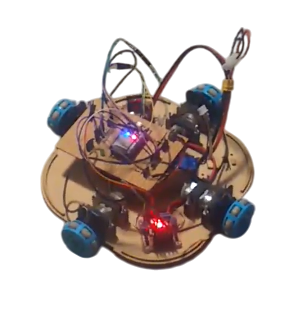
\includegraphics[trim={0 1cm 0 1cm}, clip, width=0.55\linewidth]{images/robot_sin_imanes_prototipo.png}
    \caption{Prototipo del robot}
    \label{fig:primerprototiporobot}
\end{figure}


\subsection{Riesgos superados}

En esta iteración se logro avanzar sobre el riesgo RI-03, pero para poder superarlo debemos explotar aun mas las capacidades del robot en las siguientes iteraciones.

Por otro lado, el riesgo RI-05 se logra superar en parte porque en esta iteración se incorporaron la mayoría de componentes esenciales.

\begin{center} \begin{tabular}{|p{0.10\linewidth}|p{0.65\linewidth}|}
\hline
    ID & Descripción \\
\hline
    RI-03 & Prestaciones insuficientes de componentes. \\
\hline
    RI-05 & Dificultad en conseguir determinados componentes. \\
\hline
\end{tabular} \end{center}

\subsection{Conclusiones}

En esta iteración se logró adquirir conocimientos partiendo del control individual de una rueda a modelar matemáticamente un robot teniendo en cuenta el efecto de todas las ruedas. Se obtuvo un prototipo que realiza mediciones de velocidad y distancia y las puede reportar inalámbricamente. Podemos decir que se alcanzó la meta de lograr un prototipo funcional superando varios desafíos para la cinemática y mecánica del robot.